\documentclass[a4paper, fontsize=14pt]{article}
\usepackage{style}
\setcounter{page}{0} %в зависимости от того, какой по счёту страницей должно быть оглавление!

\begin{document}

\tableofcontents

\newpage

\section*{Введение}
\addcontentsline{toc}{section}{Введение}
\newpage
% ...


\section*{Уравнение распространения волн в сейсмической среде с затуханием} 
\addcontentsline{toc}{section}{Уравнение распространения волн в сейсмической среде с затуханием}

На практике сейсмические среды с эффектом затухания описываются линейной теорией вязкоупругости.
Эта теория учитывает как упругие, так и вязкие свойства материалов,
позволяя более точно моделировать поведение материалов под воздействием сейсмических нагрузок. 
Подробную информацию можно найти в книгах \cite{Christenses,Mainardi,Carcione,Borcherdt}, здесь же ограничимся
приведением основных формул и математических формулировок в контексте задачи распространения волн.

Будем рассматривать инфинитезимальные напряжения ($\varepsilon_{ij}$) и малые перемещения ($u_{ij}$).
В этом случае они будут связаны уравнением:

\begin{equation}
    \label{eq:strain_u_rel}
    \varepsilon_{ij} = \frac{1}{2} \left( \frac{\partial u_i}{\partial x_j} + \frac{\partial u_j}{\partial x_i}\, \right). 
\end{equation}

Также будем считать, что история деформаций ($\varepsilon_{ij}(t)$) предполагается непрерывной, а функционал преобразующий историю изменения деформаций ($\varepsilon_{ij}(t)$) в соответствующую историю изменения напряжений ($\sigma_{ij}(t)$) предполагается линейным (подробнее см. \cite{Christenses})

Тогда в самом общем виде этот функционал, который будем называть определяющим уравнением, записывается следующим образом:

\begin{equation}
    \label{eq:hooks_law}
    \sigma_{ij}(t) = \int_{-\infty}^{\infty} G_{ijkl} (t - s) \frac{\partial \varepsilon_{kl} (s)}{\partial s} d s = G_{ijkl}(t) \ast  \frac{\partial \varepsilon_{kl} (t)}{\partial t} ,
\end{equation}
где $G_{ijkl}(t)$ нызывается релаксационным тензором, причем компоненты тензора $G_{ijkl}$ равны нулю при $t < 0$.

Такая запись определяющего соотношения позволяет увидеть, что оно удовлетворяет двум фундаментальным гипотезам теории линейной вязкоупругости:
\begin{enumerate}
    \item инвариантность по отношению к переносу по времени;
    \item принцип причинности (отклик системы на возмущение зависит только от предыдущих событий во времени).
\end{enumerate}

Поскольку $\sigma_{ij}$ и $\varepsilon_{ij}$ являются симметричными тензорами, то $G_{ijkl}$ также симметричный тензор: $G_{ijkl} = G_{jikl} = G_{ijlk}$.


Для изотропной среды функция релаксация имеет вид:
\begin{equation}
    \label{eq:relax_function}
    G_{ijkl} (t) = \frac{1}{3} \left( G_{b}(t) - G_{s}(t) \right) \delta_{ij} \delta_{kl} + \frac{1}{2} G_s \left( \delta_{ik} \delta_{jl} + \delta_{il} \delta_{jk}\right), 
\end{equation}
где $G_s$ и $G_b$ пространственно независимые релаксационные функции, характеризующие сдвиговые и объемные свойства материала при соответствующих деформациях; 
$\delta_{ij}$ --~  символ Кронекера;

Часто уравнение \eqref{eq:relax_function} переписывают в терминах, аналогичных константам Ламе из классической теории упругости. Для этого можно сделать замену:
\begin{equation}
    \label{eq:lame_mu}
    \hat{M}(t) = \frac{G_s(t)}{2},
\end{equation}
\begin{equation}
    \label{eq:lame_lambda}
    \hat{\Lambda}(t) = \frac{G_k(t) - G_s(t)}{3},
\end{equation}
\begin{equation}
    \label{eq:lame_pi}
    \hat{\Pi}(t) = \hat{\Lambda}(t) + 2 \hat{M}(t) .
\end{equation}

По аналогии с классической теорией упругости можно показать, что $\Pi$ является функцией релаксации для $S$ волн, а $M$ функция релаксации для $P$ волн, а
$\lambda = \pi - 2\mu$, где $\lambda, \; \pi, \; \mu$ --~ аналоги констант Ламе. 

Подставив \eqref{eq:lame_mu}, \eqref{eq:lame_lambda} в соотношение \eqref{eq:relax_function} получим:

\begin{equation}
    \label{eq:relax_tensor_lame}
    G_{ijkl}(t) = \hat{\Lambda}(t) \; \delta_{ij} \delta_{kl} + \hat{M}(t) \left( \delta_{ik} \delta_{jl} + \delta_{il} \delta_{jk}\right),
\end{equation}
а \eqref{eq:hooks_law} перепишется в виде, похожим на упругий закон Гука:
\begin{equation}
    \label{eq:hooks_law_lame}
    \sigma_{ij} = \delta_{ij} \;  \hat{\Lambda} \ast \frac{\partial \varepsilon_{kk}}{\partial t} + 2 \hat{M} \ast \frac{\partial \varepsilon_{ij}}{\partial t}.
\end{equation}

Для модели стандартного линейного тела (см. \cite{Mainardi,Carcione}), используя $\tau$-метод (см. \cite{t-method}), выводятся функции $M(t)$ и $\Pi(t)$ в виде:

\begin{equation}
    \label{eq:mu}
    \hat{M} =\mu \left[ 1 + \tau^S \exp \left( - \frac{t}{\tau} \right)\right] H (t) = M(t) H(t),
\end{equation}

\begin{equation}
    \label{eq:k}
    \hat{\Pi} = \pi \left[ 1 + \tau^P \exp \left( - \frac{t}{\tau} \right)\right] H (t) = \Pi(t) H(t),
\end{equation}
где $H(t)$ функция Хэвисайда. Также введем обозначение:
\begin{equation}
    \Lambda = \Pi - 2 M
\end{equation}

Тогда уравнение \eqref{eq:hooks_law_lame} можно переписать в виде:
\begin{equation}
    \label{eq:hooks_law_hat}
    \sigma_{ij}(t) = \delta_{ij} \int_0^t \Lambda(t - s) \; \frac{d \varepsilon_{kk}(s)}{d s} ds + 2 \int_0^t M(t - s) \; \frac{d \varepsilon_{ij}(s)}{d s} ds.  
\end{equation}

Теперь выведем дифференциальное уравнение движения в виде системы дифференциальных уравнений в частных производных 1-го порядка.

Проинтегрируем по частям \eqref{eq:hooks_law_hat}:

\begin{equation}
    \label{eq:hooks_law_int_by_part}
    \begin{aligned}
        \sigma_{ij}(t) = \; \delta_{ij} & \Lambda(0) \; \varepsilon_{kk}(t) + \delta_{ij} \int_0^t \frac{\partial \Lambda(t - s)}{\partial s}  \varepsilon_{kk}(s) ds + \\
        + & 2 M(0) \; \varepsilon_{ij}(t) + 2 \int_0^t \frac{\partial M(t - s)}{\partial s}  \varepsilon_{ij}(s) ds.
    \end{aligned}
\end{equation}


Продифференцируем \eqref{eq:hooks_law_int_by_part} по $t$:
\begin{equation}
    \label{eq:hooks_law_int_by_part_differentiate}
    \begin{aligned}
        \frac{\partial \sigma_{ij}}{\partial t}  = \; \delta_{ij} & \Lambda(0) \; \frac{\partial \varepsilon_{kk}}{\partial t}  + \delta_{ij} \frac{d}{dt} \int_0^t \frac{\partial \Lambda(t - s)}{\partial s}  \varepsilon_{kk}(s) ds + \\
        + & 2 M(0) \; \frac{\partial \varepsilon_{ij}}{\partial t} + 2 \frac{d}{dt} \int_0^t \frac{\partial M(t - s)}{\partial s}  \varepsilon_{ij}(s) ds 
    \end{aligned}
\end{equation}

Заметим, что:
\begin{equation}
    \label{eq:mu_t}
    \frac{d M}{d t} = - \frac{\mu}{\tau} \tau^S \exp \left( - \frac{t}{\tau}\right), \; \text{и} \;  \frac{d^n M}{d^n t} = (-1)^{n-1} \frac{1}{\tau^{n-1}} \frac{d M}{d t}, \; n \geq 2. 
\end{equation}

Аналогично,
\begin{equation}
    \label{eq:k_t}
    \frac{d \Pi}{d t} = - \frac{\pi}{\tau} \tau^P \exp \left( - \frac{t}{\tau}\right)  \; \text{и} \;  \frac{d^n \Pi}{d^n t} = (-1)^{n-1} \frac{1}{\tau^{n-1}} \frac{d \Pi}{dt}, \; n \geq 2. 
\end{equation}



Введем новые переменные:
\begin{equation*}
    \begin{aligned}
        r_{ij} &= \delta_{ij} \; \frac{d}{dt} \int_0^t \frac{\partial \Lambda(t - s)}{\partial s}  \varepsilon_{kk}(s) ds + 2 \frac{d}{dt} \int_0^t \frac{\partial M(t - s)}{\partial s}  \varepsilon_{ij}(s) ds = \\
           & = \delta_{ij} \left[\; \frac{d \Lambda}{d t}\Big{|}_{t = 0} \;  \; \varepsilon_{kk} (t) + \int_0^t \frac{\partial^2 \Lambda(t - s)}{\partial^2 s} \varepsilon_{kk}(s) ds \right] + \\ 
           & + 2 \left[ \frac{d M}{d t}\Big{|}_{t = 0} \;  \varepsilon_{ij} + \int_0^t \frac{\partial^2 M(t - s)}{\partial^2 s} \varepsilon_{ij}(s) ds \right] 
    .\end{aligned}
\end{equation*}

Используя \eqref{eq:mu_t} и \eqref{eq:k_t} можно записать:

\begin{equation}
    \label{eq:r_rare}
    \begin{aligned}
        r_{ij} &= \delta_{ij} \left[\; \frac{d \Lambda}{d t}\Big{|}_{t = 0} \;  \; \varepsilon_{kk} (t) - \frac{1}{\tau} \int_0^t \frac{\partial \Lambda(t - s)}{\partial s} \varepsilon_{kk}(s) ds \right] + \\ 
           & + 2 \left[ \frac{d M}{d t}\Big{|}_{t = 0} \;  \varepsilon_{ij} - \frac{1}{\tau} \int_0^t \frac{\partial M(t - s)}{\partial s} \varepsilon_{ij}(s) ds \right].
    \end{aligned}
\end{equation}

Продифференцируем \eqref{eq:r_rare} по времени:

\begin{equation*}
    \begin{aligned}
        \frac{d r_{ij}}{dt} &= \delta_{ij} \left[\; \frac{d \Lambda}{d t}\Big{|}_{t = 0} \;  \; \frac{d \varepsilon_{kk}}{dt}  (t) - \frac{1}{\tau} \frac{d}{dt} \int_0^t \frac{\partial \Lambda(t - s)}{\partial s} \varepsilon_{kk}(s) ds \right] + \\ 
           & + 2 \left[\frac{d M}{d t}\Big{|}_{t = 0} \; \frac{d \varepsilon_{ij}}{dt}  - \frac{1}{\tau} \frac{d}{dt} \int_0^t \frac{\partial M(t - s)}{\partial s} \varepsilon_{ij}(s) ds \right].
    \end{aligned}
\end{equation*}

Теперь имеем два случая:
\begin{equation}
    \label{eq:memory_funct}
    \begin{aligned}
        1.& \; i = j \Rightarrow \tau \frac{dr_{ii}}{dt} =  -  \left(\pi \tau^P - 2 \mu \tau^S \right) \frac{d \varepsilon_{kk}}{dt} -\, 2\mu \tau^S \frac{d \varepsilon_{ii}}{dt} -  r_{ii} \\
        2.& \; i \neq j \Rightarrow \tau \frac{dr_{ij}}{dt} = - 2 \mu \tau^S \frac{d \varepsilon_{ij}}{dt} - r_{ij} 
    \end{aligned}
\end{equation}

Переменные $r_{ij}$ отвечают за историю процесса, поэтому называются функциями памяти. Благодаря им уравнение \eqref{eq:hooks_law_int_by_part_differentiate} будет иметь вид:
\begin{equation}
    \label{eq:hooks_law_final}
    \begin{aligned}
        \frac{\partial \sigma_{ij}}{\partial t}  = \; \delta_{ij} \left(\pi (\tau^P + 1) - 2 \mu (\tau^S + 1) \right)  \frac{\partial \varepsilon_{kk}}{\partial t} + 2 \mu (\tau^S + 1)  \frac{\partial \varepsilon_{ij}}{\partial t} + r_{ij}
    \end{aligned}
\end{equation}

Запишем уравнение баланса импульса для сплошной среды: 
\begin{equation}
    \label{eq:newton_law}
    \rho \frac{\partial^2 u_{i}}{\partial^2 t} = \frac{\partial \sigma_{ij}}{\partial x_j}  + f_{i} \quad \text{или} \quad \rho \frac{\partial v_{i}}{\partial t}  = \frac{\partial \sigma_{ij}}{\partial x_j}  + f_{i},
\end{equation}
где $u_{i}, v_{i}$ компоненты векторов перемещения и скорости перемещения, $\sigma_{ij}$ компонент симметричного тензора напряжения, $f_i$ компонент вектора внешних массовых сил, $\rho$ плотность среды.

Таким образом, подставив в \eqref{eq:memory_funct}, \eqref{eq:hooks_law_final} продифференцированное по времени соотношение \eqref{eq:strain_u_rel}, будем иметь замкнутую систему дифференциальных уравнений \eqref{eq:memory_funct}, \eqref{eq:hooks_law_final} и \eqref{eq:newton_law}, описывающую движение в вязкоупругой среде.
Эту систему можно представить в следующим виде:
\begin{equation}
    \label{eq:system_on_v}
    \renewcommand\arraystretch{1.6}
    \frac{\partial }{\partial t}\, 
    \begin{pmatrix}
        v_1 \\
        v_2 \\
        v_3
    \end{pmatrix} =
    \frac{1}{\rho} 
    \begin{pmatrix} 
        \frac{\partial \sigma_{11}}{\partial x_1} +  \frac{\partial \sigma_{12}}{\partial x_2} + \frac{\partial \sigma_{13}}{\partial x_3} \\
        \frac{\partial \sigma_{21}}{\partial x_1} +  \frac{\partial \sigma_{22}}{\partial x_2} + \frac{\partial \sigma_{23}}{\partial x_3}\, \\
        \frac{\partial \sigma_{31}}{\partial x_1} +  \frac{\partial \sigma_{32}}{\partial x_2} + \frac{\partial \sigma_{33}}{\partial x_3}
    \end{pmatrix},
\end{equation}
\begin{equation}
    \label{eq:system_on_sigma}
    \renewcommand\arraystretch{1.6}
    \frac{\partial }{\partial t}\, 
    \begin{pmatrix}
        \sigma_{11} \\
        \sigma_{22} \\
        \sigma_{33} \\
        \sigma_{23} \\
        \sigma_{13} \\
        \sigma_{12}
    \end{pmatrix} = A_1
    \begin{pmatrix} 
    \frac{\partial u_1}{\partial x_1} \\
    \frac{\partial u_2}{\partial x_2} \\
    \frac{\partial u_3}{\partial x_3} \\
    \frac{\partial u_2}{\partial x_3} + \frac{\partial u_3}{\partial x_2} \\
    \frac{\partial u_3}{\partial x_1} + \frac{\partial u_1}{\partial x_3} \\
    \frac{\partial u_1}{\partial x_2} + \frac{\partial u_2}{\partial x_1}
    \end{pmatrix} +
    \begin{pmatrix} 
    r_{11} \\
    r_{22} \\
    r_{33} \\
    r_{23} \\
    r_{12} \\
    r_{12} 
    \end{pmatrix},
\end{equation}

\begin{equation}
    \label{eq:system_on_r}
    \renewcommand\arraystretch{1.6}
    \tau \frac{\partial }{\partial t}
    \begin{pmatrix} 
        r_{11} \\
        r_{22} \\
        r_{33} \\
        r_{23} \\
        r_{12} \\
        r_{12} 
    \end{pmatrix} 
    = - A_2 
    \begin{pmatrix} 
        \frac{\partial u_1}{\partial x_1} \\
        \frac{\partial u_2}{\partial x_2} \\
        \frac{\partial u_3}{\partial x_3} \\
        \frac{\partial u_2}{\partial x_3} + \frac{\partial u_3}{\partial x_2} \\
        \frac{\partial u_3}{\partial x_1} + \frac{\partial u_1}{\partial x_3} \\
        \frac{\partial u_1}{\partial x_2} + \frac{\partial u_2}{\partial x_1}
        \end{pmatrix} -
        \begin{pmatrix} 
        r_{11} \\
        r_{22} \\
        r_{33} \\
        r_{23} \\
        r_{12} \\
        r_{12} 
        \end{pmatrix},
\end{equation}

Заменив в \eqref{eq:memory_funct}, \eqref{eq:hooks_law_final} значение $\pi$ на $\lambda + 2 \mu$, можно заметить, что матрицы $A_1$ и $A_2$ имеют вид:
\begin{equation}
    A_i = 
    \begin{pmatrix}
        a_i^P & a_i & a_i & 0 & 0 & 0 \\ 
        a_i & a_i^P & a_i & 0 & 0 & 0 \\ 
        a_i & a_i & a_i^P & 0 & 0 & 0 \\ 
        0 & 0 & 0  & a_i^S & 0 & 0 \\
        0 & 0 & 0  & 0  & a_i^S & 0 \\
        0 & 0 & 0  & 0 & 0 & a_i^S
    \end{pmatrix},
    \quad
    \text{где}
    \quad
    \begin{aligned}
        a_1^P &= (\lambda + 2 \mu) (1 + \tau^P) \\
        a_1^S &= \mu(1 + \tau^S) \\
        a_i &= a_i^P - 2 a_i^S \\
        a_2^P &= (\lambda + 2 \mu) \tau^P \\
        a_2^S &= \mu \tau^S
    \end{aligned}
\end{equation}


\section*{Разностная аппроксимация. Схема на смещенной сетке} 
\addcontentsline{toc}{section}{Разностная аппроксимация. Схема на смещенной сетке} 

В работах \cite{Bohlen,Levander} для аппроксимации системы ДУЧП \eqref{eq:system_on_v}, \eqref{eq:system_on_sigma}, \eqref{eq:system_on_r} используются схема на основе следующих разностных  аппроксимаций:

\begin{equation}
    \label{eq:fd_time}
    D_{t}[f]_{I,J,K}^{N}=\frac{f_{I,J,K}^{N+1/2}-f_{I,J,K}^{N-1/2}}{d t}=\frac{\partial f}{\partial t}\bigg|_{I,J,K}^{N}+O(d t^{2})
\end{equation}

\begin{equation}
    \label{eq:fd_f}
    A_{t}[f]_{I,J,K}^{N+1/2}=\frac{f_{I,J,K}^{N+1/2}+f_{I,J,K}^{N-1/2}}{2}=f_{I,J,K}^{N}+O(d t^{2})
\end{equation}


\begin{equation}
    \label{eq:fd_space}
    D_{1}[f]_{I,J,K}^{N}=\sum_{m=1}^{M}\alpha_{m}\frac{f_{I+m-1/2,J,K}^{N}-f_{I-m+1/2,J,K}^{N}}{h_{1}}=\frac{\partial f}{\partial x_{1}}\bigg|_{I,J,K}^{N}+O(h_{1}^{2m}).
\end{equation}

В этих обозначениях индексы, написанные заглавными буквами, могут быть как целыми, так и полуцелыми, $dt$ шаг
временой сетки, $h_1, h_2, h_3$ шаги пространственной сетки. Дополнительный параметр $M$ определяет длину
шаблона и коэффициенты $\alpha_m$ используются для достижения необходимого порядка аппроксимации.
Значения вплоть до 10 порядка аппроксимации приведены в таблице 1. Программа для расчета данных коэффициентов для любого $M$ приведена в приложении.

\begin{table}[htbp]
    \centering
    \begin{tabular}{|c|c|c|c|c|c|}
        \hline
        $M$ & $\alpha_0$ & $\alpha_1$ & $\alpha_2$ & $\alpha_3$ & $\alpha_4$\\
        \hline
        1 & 1.0 & & & & \\
        \hline
        2 & 9/8 & -1/24 & & & \\
        \hline
        3 & 75/64 & -25/384 & 3/640 & & \\
        \hline
        4 & 1125/1024 & -245/3072 & 49/5120 & -5/7168 & \\
        \hline
        5 & 19845/16384 & -735/8192& 567/40960 & -405/229376 & 35/294912 \\
        \hline
    \end{tabular}
    \caption{Коэффициенты аппроксимации \eqref{eq:fd_space} для различных M}
    \label{tab:mytable}
\end{table}

Аналогично \eqref{eq:fd_space} можно ввести аппроксимации и для других пространственных перменных.

Тогда разностный аналог для системы \eqref{eq:system_on_v}, \eqref{eq:system_on_sigma}, \eqref{eq:system_on_r}  будет иметь следующий вид:
%\begin{equation*}
    \begin{gather*}
        \rho D_{t}[u_{1}]_{I,J,K}^{n-1/2} = D_{1}[\sigma_{11}]_{I,J,K}^{n-1/2}+D_{2}[\sigma_{12}]_{I,J,K}^{n-1/2}+D_{3}[\sigma_{13}]_{I,J,K}^{n-1/2},\\ \text{где } \{I,J,K\}=\{i+1/2,j,k\},\\ 
        \rho D_{t}[u_{2}]_{I,J,K}^{n-1/2} = D_{1}[\sigma_{12}]_{I,J,K}^{n-1/2}+D_{2}[\sigma_{22}]_{I,J,K}^{n-1/2}+D_{3}[\sigma_{23}]_{I,J,K}^{n-1/2},\\ \text{где } \{I,J,K\}=\{i,j+1/2,k\},\\ 
        \rho D_{t}[u_{3}]_{I,J,K}^{n-1/2} = D_{1}[\sigma_{13}]_{I,J,K}^{n-1/2}+D_{2}[\sigma_{23}]_{I,J,K}^{n-1/2}+D_{3}[\sigma_{13}]_{I,J,K}^{n-1/2},\\ \text{где } \{I,J,K\}=\{i,j,k+1/2\},\\ 
        D_{t}[\sigma_{11}]_{I,J,K}^{n} = p_{1}^{P}D_{1}[u_{1}]_{I,J,K}^{n}+p_{1}^{d}D_{2}[u_{2}]_{I,J,K}^{n}+p_{1}^{d}D_{3}[u_{3}]_{I,J,K}^{n}+\sum_{l=1}^{L}A_{t}[r_{1,l}]_{I,J,K}^{n}, \\ \text{где }\{I,J,K\}=\{i,j,k\},\\ 
        D_{t}[\sigma_{22}]_{I,J,K}^{n} = p_{1}^{P}D_{1}[u_{1}]_{I,J,K}^{n}+p_{1}^{d}D_{2}[u_{2}]_{I,J,K}^{n}+p_{1}^{d}D_{3}[u_{3}]_{I,J,K}^{n}+\sum_{l=1}^{L}A_{t}[r_{1,l}]_{I,J,K}^{n}, \\ \text{где }\{I,J,K\}=\{i,j,k\},\\ 
        D_{t}[\sigma_{33}]_{I,J,K}^{n} = p_{1}^{P}D_{1}[u_{1}]_{I,J,K}^{n}+p_{1}^{d}D_{2}[u_{2}]_{I,J,K}^{n}+p_{1}^{d}D_{3}[u_{3}]_{I,J,K}^{n}+\sum_{l=1}^{L}A_{t}[r_{1,l}]_{I,J,K}^{n}, \\ \text{где }\{I,J,K\}=\{i,j,k\},\\ 
        D_{t}[\sigma_{23}]_{I,J,K}^{n}=p_{1}^{S}D_{3}[u_{2}]_{I,J,K}^{n}+p_{1}^{S}D_{2}[u_{3}]_{I,J,K}^{n}+\sum_{l=1}^{L}A_{t}[r_{23,l}]_{I,J,K}^{n}, \\ \text{где } \{I,J,K\}=\{i,j+1/2,k+1/2\},\\ 
        D_{t}[\sigma_{13}]_{I,J,K}^{n}=p_{1}^{S}D_{1}[u_{3}]_{I,J,K}^{n}+p_{1}^{S}D_{3}[u_{1}]_{I,J,K}^{n}+\sum_{I=1}^{L}A_{t}[r_{13,l}]_{I,J,K}^{n}, \\ \text{где } \{I,J,K\}=\{i+1/2,j,k+1/2\},\\ 
        D_{t}[\sigma_{12}]_{I,J,K}^{n}=p_{1}^{S}D_{2}[u_{1}]_{I,J,K}^{n}+p_{1}^{S}D_{1}[u_{2}]_{I,J,K}^{n}+\sum_{l=1}^{L}A_{t}[r_{12,l}]_{I,J,K}^{n}, \\ \text{где } \{I,J,K\}=\{i+1/2,j+1/2,k\},\\ 
        \tau D_{t}[r_{11}]_{I,J,K}^{n}=-p_{2}^{P}D_{1}[u_1]_{I,J,K}^{n}-p_{2}^{d}D_{2}[u_{2}]_{I,J,K}^{n}-p_{2}^{d}D_{3}[u_{3}]_{I,J,K}^{n}  - A_{t}[r_{11}]_{I,J,K}^{n}, \\ \text{где }\{I,J,K\}=\{i,j,k\},\\ 
        \tau D_{t}[r_{22}]_{I,J,K}^{n}=-p_{2}^{d}D_{1}[u_{1}]_{I,J,K}^{n}-p_{2}^{P}D_{2}[u_{2}]_{I,J,K}^{n}-p_{2}^{d}D_{3}[u_{3}]_{I,J,K}^{n}- A_{\ell}[r_{22}]_{I,J,K}^{n}, \\ \text{где }\{I,J,K\}=\{i,j,k\},\\ 
        \tau D_{t}[r_{33}]_{I,J,K}^{n}=-p_{2}^{d}D_{1}[u_{1}]_{I,J,K}^{n}-p_{2}^{d}D_{2}[u_{2}]_{I,J,K}^{n}-p_{2}^{P}D_{3}[u_{3}]_{I,J,K}^{n}- A_{t}[r_{32}]_{I,J,K}^{n}, \\ \text{где }\{I,J,K\}=\{i,j,k\},\\ 
    \end{gather*}

    \begin{gather*}
        \tau D_{t}[r_{23}]_{t,J,K}^{n}=-p_{2}^{S}D_{3}[u_{2}]_{t,J,K}^{n}-p_{2}^{S}D_{2}[u_{3}]_{t,J,K}^{n}-A_{t}[r_{23}]_{I,J,K}^{n},\\ \text{где }\{I,J,K\}=\{i,j+1/2,k+1/2\},\\ 
        \tau D_{t}[r_{13}]_{I,J,K}^{n}=-p_{2}^{S}D_{1}[u_{3}]_{I,J,K}^{n}-p_{2}^{S}D_{3}[u_{1}]_{I,J,K}^{n}-A_{t}[r_{13}]_{I,J,K}^{n},\\ \text{где }\{I,J,K\}=\{i+1/2,j,k+1/2\},\\ 
        \tau D_{t}[r_{12}]_{I,J,K}^{n}=-p_{2}^{S}D_{2}[u_{1}]_{I,J,K}^{n}-p_{2}^{S}D_{1}[u_{2}]_{I,J,K}^{n}-A_{t}[r_{12}]_{I,J,K}^{n},\\ \text{где }\{I,J,K\}=\{i+1/2,j+1/2,k\}.\\ 
    \end{gather*}

В \cite{Bohlen} приведено число Куранта для вышеприведенной схемы:

\begin{equation}
    c_{p}^{\mathrm{Umax}} \cdot  dt \cdot \sqrt{\frac{1}{dx^2} + \frac{1}{dy^2}  + \frac{1}{dz^2} } < 1,
\end{equation}
где $c_{p}^{\mathrm{Umax}}$ константа, задающее начальное распеделение скорости P-волн в вакууме.

Для двумерного случая программная реализация схемы на языке Julia приведена в приложении.

\section*{Поглощающий граничный слой для схемы на смещенной сетке} 
\addcontentsline{toc}{section}{Поглощающий граничный слой для схемы на смещенной сетке}

Для численного исследования задач распространения волны в неграниченной области используется техника идеально поглощающих слоев, называемых PML (perfectly matched layer). Схема показана на рисунке 1.

\begin{figure}[h!]
    \begin{center}
        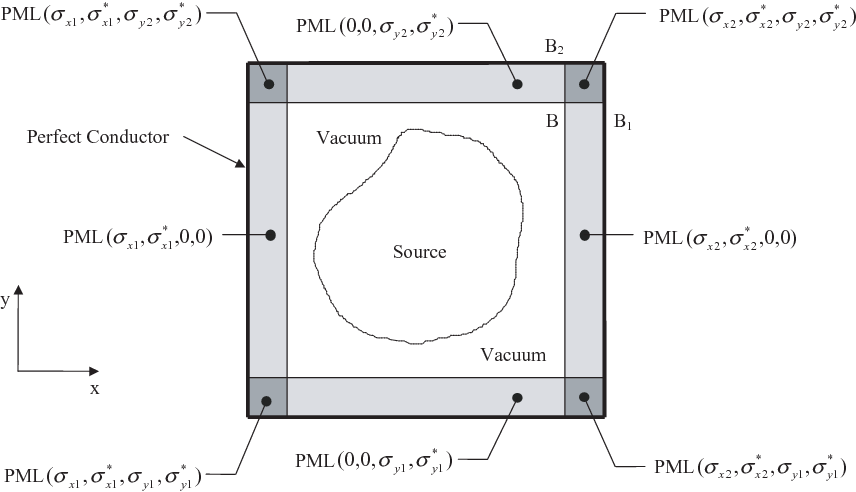
\includegraphics[width=15cm]{./assets/pml.png}    
    \end{center}
    \caption{Схема идеально поглощающего слоя}
\end{figure}

Классический подход к построению PML для системы уравнений типа  \eqref{eq:system_on_v}, \eqref{eq:system_on_sigma}, \eqref{eq:system_on_r} рассмотрен в статье \cite{Collino}.
Однако, существует подход (см., например, \cite{Martin}), в котором приводится формулировка, требующая значетельно меньше памяти, но эквивалентная классическому подходу в математическом смысле.
Такой подход получил название сверточного идеально поглощающего слоя CPML (convolutional PML).

Его суть заключается в замене пространственной производной:

\begin{equation}
    \frac{\partial}{\partial x_i} \rightarrow \frac{1}{\kappa_{x_i}}\frac{\partial}{\partial x_i} + \psi_{x_i},
\end{equation}
а функция $\psi_{x_i}$ (в районе $x_i$ = 0) определяется с помощью следующей цепочки уравнений (подробнее см. \cite{Martin}):
\begin{equation}
    \psi_{x_i}^{n}(f)=b_{x_i}\psi_{x_i}^{n-1}(f)+a_{x_i}\left(\partial_{x_i}f\right)^{n-1/2},
\end{equation}

\begin{equation}
    \label{eq:bxi}
    b_{x_i}=e^{-(d/\kappa_{x_i}+\alpha_{x_i})\Delta t},
\end{equation}

\begin{equation}
    a_{x_i}=\frac{d_{x_i}}{\kappa_{x_i}(d_{x_i}+\kappa_{x_i}\alpha(x_i))}(b_{x_i}-1),
\end{equation}

\begin{equation}
    d(x_i)\,=\,d_{0}\left(1 - \frac{x_i}{L}\right)^{2}
\end{equation}

\begin{equation}
    d_{0}=-{\frac{3 c_{p}^{\mathrm{Umax}}\log(R_{c})}{2 L}}
\end{equation}

\begin{equation}
    \kappa_{x_{i}}=1+(\kappa_{\operatorname*{max}}-1)\left(1 - \frac{x_{i}}{L}\right)^{2}
\end{equation}

\begin{equation}
    \label{eq:alphaxi}
    \alpha(x_i) = \alpha_{\operatorname*{max}} \left(\frac{x_i}{L}\right)^2
\end{equation}

Здесь $\Delta t$ шаг про времени, $L$ - размер PML области, 
$c_{p}^{\mathrm{Umax}}$ константа, задающее начальное распеделение скорости P-волн в вакууме, 
$R_c$ - теоретический коэффициент отражения от границы слоя
$\kappa_{\operatorname*{max}}$ и $\alpha_{\operatorname*{max}}$ определяются произвольно и требуют дополнительного изучения.

На противоположном от $x_i = 0$ конце расчетной области \eqref{eq:bxi}-\eqref{eq:alphaxi} задаются аналогично, но в обратном направлении. Подробная программная реализация в двумерном случае приведена в приложении.

\section*{Результаты программной реализации} 
\addcontentsline{toc}{section}{Результаты программной реализации}


\newpage
\section*{Заключение}
\addcontentsline{toc}{section}{Заключение}

\newpage


\begin{thebibliography}{9}
    \addcontentsline{toc}{section}{\refname}
    \bibitem{Christenses} Введение в теорию вязкоупругости / Р. Кристенсен ; пер. с англ. М. И. Рейтмана ; под ред. Г. С. Шапиро, 1974. - 338 с
    \bibitem{Mainardi} Fractional Calculus and Waves in Linear Viscoelasticity
    \bibitem{Carcione} Wave in real solid
    \bibitem{Borcherdt} Viscoelastic waves and rays in layered media
    \bibitem{Bohlen} T. Bohlen, “Parallel 3-D viscoelastic finite difference seismic modelling,” Comput. Geosci. 28, 887–899
    \bibitem{t-method} Blanch, J. O., Robertsson, J. O. A.,  Symes, W. W. (1995). Modeling of a constantQ: Methodology and algorithm for an efficient and optimally inexpensive viscoelastic technique. 
    (2002).
    \bibitem{Levander} A. R. Levander, “Fourth-order finite-difference P-SV seismograms,
    \bibitem{Collino} Collino, F. Tsogka, C., 2001. Application of the PML absorbing layer
    model to the linear elastodynamic problem in anisotropic heterogeneous
    media, Geophysics, 66(1), 294–307.
    \bibitem{Martin} Martin, R.,  Komatitsch, D. (2009). An unsplit convolutional perfectly matched layer technique improved at grazing incidence for the viscoelastic wave equation.
\end{thebibliography}

\end{document}